\scanpage{18}
8) Soit maintenant $\mathcal E^*$ un anneau gradué, \deleted{muni de} tel qu'il existe $L\in\mathcal E^{(2)}$ satisfaisant aux \uline{conditions de Lefschetz} (\deleted{de} les conditions du corollaire du n\textsuperscript{o} précédent). On dit que $\mathcal E^*$ est un ``anneau \deleted{d'opérateurs Lefschetzien,}\inserted{de correspondances Lefschetzien}'' (\unsure{cette} \deleted{\illegible{3}} \deleted{\unsure{avec le système}} \unsure{au n\textsuperscript{o}} \unsure{(pair)} \unsure{qu'un système de|qui un système de} Lefschetz), et $L$ un de ses ``éléments de Lefschetz''.
\deleted{\unsure{En dehors} $(\unsure{\varphi(\Phi)=\mathcal E^*})$}
L'élt $\Lambda$ associé est \deleted{\unsure{dit}} \unsure{``}l'élément \deleted{\unsure{adjoint pour}} \deleted{\unsure{anti}}\inserted{co.}Lefschetzien'' associé à $L$.
(NB. À noter que $L$ se déduit de $\Lambda$ comme $\Lambda$ de $L$, par simple symétrie sur les degrés de $\mathcal E^*$ \deleted{$\unsure{\xi_0}$} $\unsure{-}$, et passage à l'anneau opposé --- \deleted{\unsure{transposé}} isom de transposition ---).
\margin{\figure{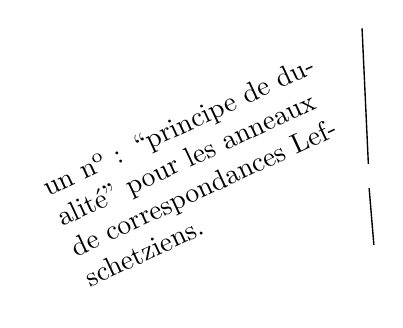
\begin{tikzpicture}
\node[align=left,text width=3.8cm,rotate=25] at (0,0) {un n\textsuperscript{o} : ``principe de dualité'' pour les anneaux de correspondances Lefschetziens.};
\draw[line width=.5pt] (2.05,1.8)--(2.13,.08);
\draw[line width=.5pt] (2.14,-.23)--(2.2,-.95);
\end{tikzpicture}}}

On peut se demander de \uline{caractériser} les \deleted{les} éléments de Lefschetz $L$. Une condition nécessaire, lorsque le \unsure{nombre} $2n$ n'est pas redondant, i.e.
\[
\begin{aligned}
1)\quad&\mathcal E^{(2n)}\neq0\quad\deleted{\unsure{\{}}\quad(\Longleftrightarrow)\quad1')\ \mathcal E^{(-2n)}\neq0\quad\deleted{\unsure{\}}}\\
&(\Longleftrightarrow)\quad2)\ \pi_0,\deleted{\unsure{\pi_{2n}}}\neq0\quad\deleted{\unsure{\}}}
\end{aligned}
\]
\margin{\figure{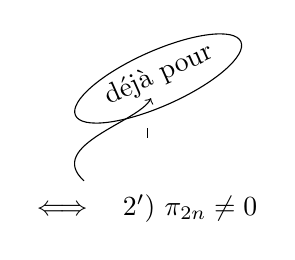
\begin{tikzpicture}
\node[align=left] at (0,0) {$\Longleftrightarrow\quad2')\ \pi_{2n}\neq0$};
\node[rotate=24] at (.15,1.7) {\unsure{déjà pour}};
\draw[rotate=24] (.8,1.45) ellipse (1.15cm and .35cm);
\draw[->] (-.8,.35) .. controls (-1.3,.8) and (-.1,1.1) .. (.05,1.4);
\draw (.01,1.02)--(.01,.9);
\end{tikzpicture}}}
que
\[
(\Longleftrightarrow)\quad3)\ L^n\neq0\quad(\Longleftrightarrow)\quad3')\ \Lambda^{\unsure{n|-}}\neq0\quad\deleted{\Longleftrightarrow}
\]
c'est que l'on ait $L^n\neq0$. On a parfois une réciproque, dans le cas où ($\mathcal E$ étant une \uline{algèbre} sur un anneau commutatif $k$)
\mspage{17}
